% ============================ Enrico Ribiani 16-03-2021 ====================================================================
% Base per i documenti  
\documentclass[12pt]{article}
% ------------ pacchetti necessari ----------------
\usepackage[a4paper, total={6in, 8in},margin=1in]{geometry} % formattazione decente della pagina
\usepackage{graphicx}                            % need for figure
\usepackage{amsmath}
\usepackage{amsfonts}                            % if you want the fonts
\usepackage{amssymb}                             % if you want extra symbols
\usepackage{graphicx}  
\renewcommand{\figurename}{Figura}  
\renewcommand{\contentsname}{Indice}                        % need for figures
\usepackage{mathptmx}
\usepackage{float}                               % serve per mettere tabelle e immagini dove si vuole 
\usepackage[utf8]{inputenc}
\usepackage{textcomp}
\usepackage[hang,flushmargin,bottom]{footmisc}   % footnote format
\usepackage{fancyhdr, lastpage}
\usepackage{titlesec}
\usepackage[table,dvipsnames]{xcolor}
%\pagestyle{fancy}
%\renewcommand{\headrulewidth}{0pt}
%\renewcommand*\contentsname{Indice}
\titleformat{\section}{\normalsize\bfseries}{\thesection.}{1em}{}	% required for heading numbering style
\titleformat*{\section}{\Large\bfseries}
\titleformat*{\subsection}{\large\bfseries}
%\usepackage{siunitx}
%\usepackage{tikz}
\usepackage{circuitikz}
\usepackage{multicol}
%\usepackage[siunitx]{circuitikz}
\usepackage{multirow}
\usepackage{tikz}
\usepackage{amsmath}
\usetikzlibrary{angles,quotes}
\usepackage{placeins}
\usepackage{tabularx,ragged2e,booktabs,caption}

\usepackage{wasysym}
%===================links=================
\usepackage{hyperref}
\hypersetup{
    colorlinks=true,
    linkcolor=darkgray,
    filecolor=Green,      
    urlcolor=Cyan,
    pdftitle={SAMPLE},
    pdfpagemode=FullScreen,
    }
%===================inizio pagina del titolo=================
\begin{document}
    \begin{titlepage}
    \begin{center}
% ------------------ inizio immagine logo ----------
\begin{figure}
    \centering
    
\includegraphics{~/varie/logo.png}
    \label{fig:logo}
\end{figure}
% ------------------ fine immagine logo ----------
% ------------------ fine immagine logo ----------
-------------------------------------------------------------------------------------\\
\vspace{4\baselineskip}


\large Prova n°1
\hfill
\large $5^a$   AUB\\

\Large Gruppo:\\
\large Enrico Ribiani\\
\large Daniel Graziadei\\


\vfill

\Huge{\textbf{Amplificatore invertente e non invertente}}\\
\vfill
\vfill
\large{22-09-2022}
\end{center}
%=============== fine pagina titolo ===============

\end{titlepage}
\tableofcontents
\newpage
\section{Scopo}
Lo scopo di questa esperienza laboratoriale è di misurare e verificare la corrispondenza tra
il guadagno di tensione misurato sperimentalmente e quello calcolato tramite calcoli teorici.\\
\section{Schema}
\begin{flushleft}
    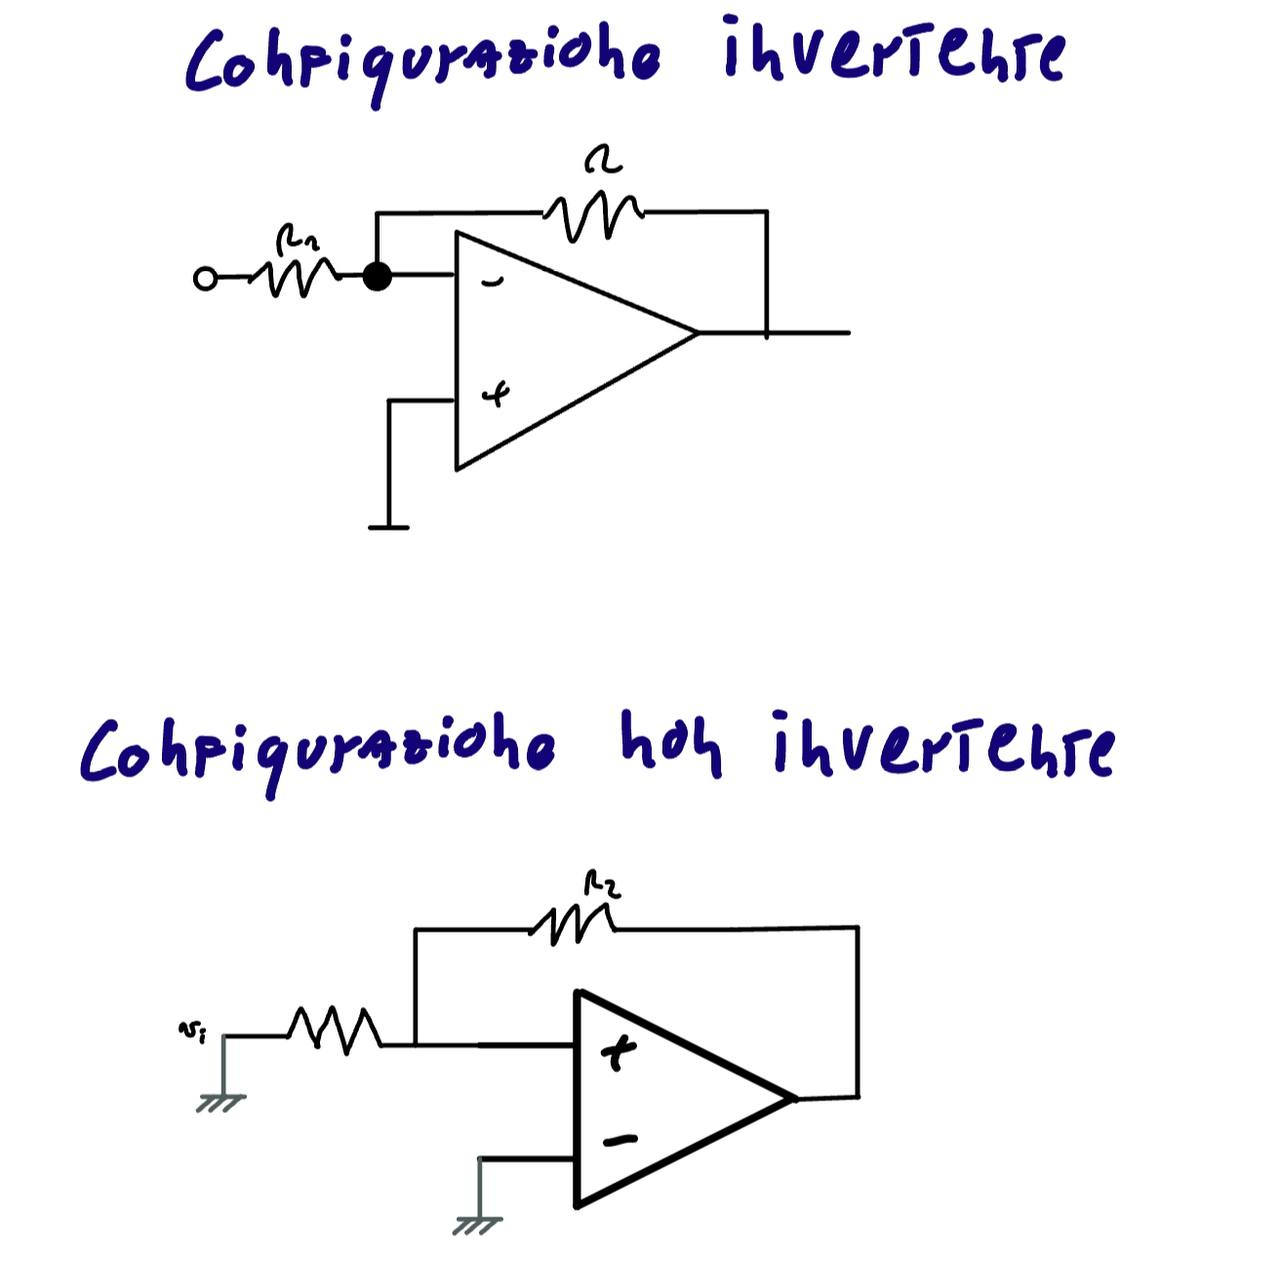
\includegraphics[scale=0.28]{Schema.jpg}
\end{flushleft}

\section{Materiale e Strumenti}
\label{Materiale e Strumenti}
\begin{multicols}{2}
    \begin{itemize}
    \item Fili di collegamento
    \item Breadboard
    \item Resistenza da $10k\Omega$
    \item Resistenza da $100k\Omega$
    \item Amplificatore operazionale \textit{U741}
    \end{itemize}
    \vfill\null
    \columnbreak
    \begin{itemize}
    \item Multimetro
    \item Generatore di funzione
    \item Oscilloscopio
    \item Alimentazione DC 
    \end{itemize}
    \vfill\null
    \end{multicols}
\vspace{15pt}
\section{Contenuti Teorici}
Avendo come dati $R_1$,$R_2$  $V_{cc}$ , $V_{iM}$, e la frequenza possiamo andare a calcolare
teoricamente quanto dovrebbe riusultare il guadagno di tensione $A_v$ tramite la formula
$A_v=-\frac{R_2}{R_1}$ per la configurazione invertente e $A_v=1+\frac{R_2}{R_1}$.\\
Andando a verificare il guadagno in modo sperimentale tramite il rapporto tra $V_i$ e $V_u$
si presuppone che i due risultati siano circa uguali.\\
\section{Descrizione della Prova}
Dopo aver svolto i calcoli teorici vanno misurate le resistenze e verificato che il valore sia 
comparabile a quello riportato tramite codice colore.\\
Dopodichè viene montato il circuito sulla Breadboard seguendo lo schema, prima di collegarlo all'
alimentazione viene regolata usando un multimetro come riferimento.
Come ultima cosa si collega e si impostano oscilloscopio e generatore di funzione.
Si misurano quindi i valori di $V_i$ e di $V_o$ tramite la funzione \textit{Measure} dell'oscilloscopio
e si annotano in tabella.\\
Si ripete la procedura per entrambe le configurazioni.\\
\section{Raccolta dei dati}
\begin{figure}[h]
    \centering
    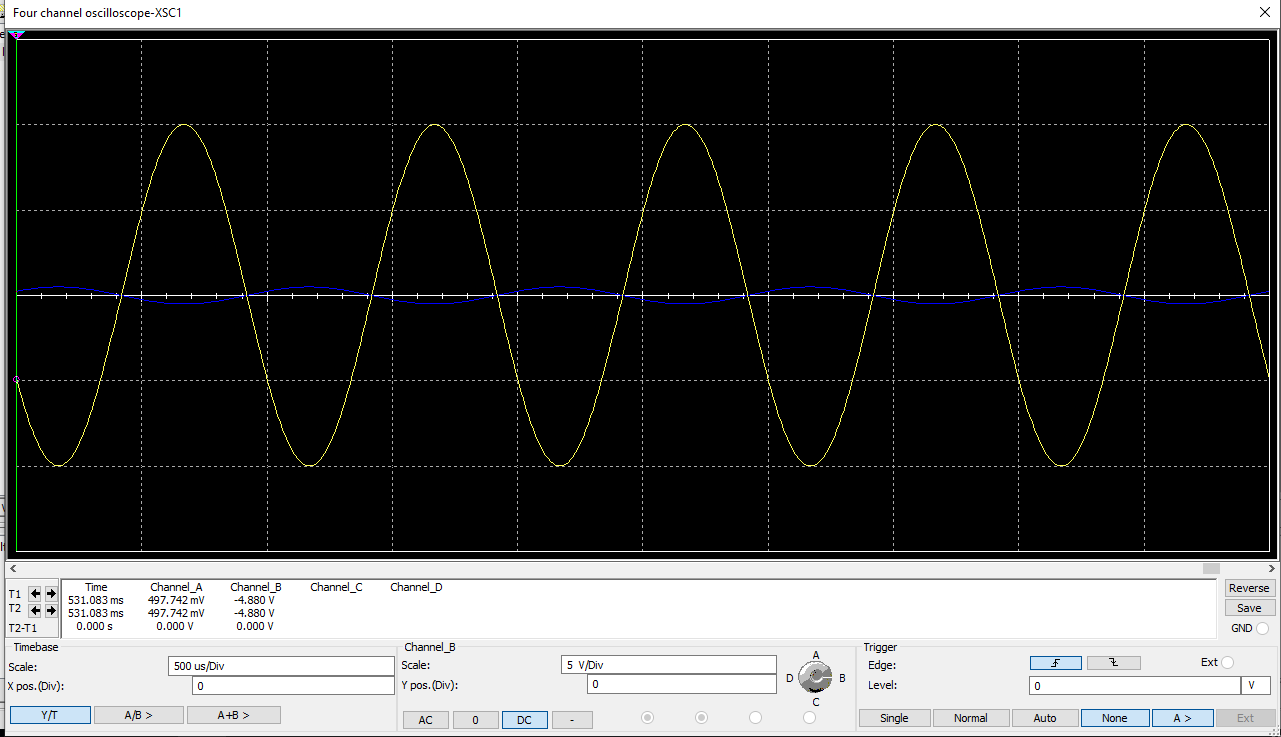
\includegraphics[scale=0.2]{aoinv.png}
    \caption{Amplificatore invertente}
\end{figure}
\begin{figure}[h]
    \centering
    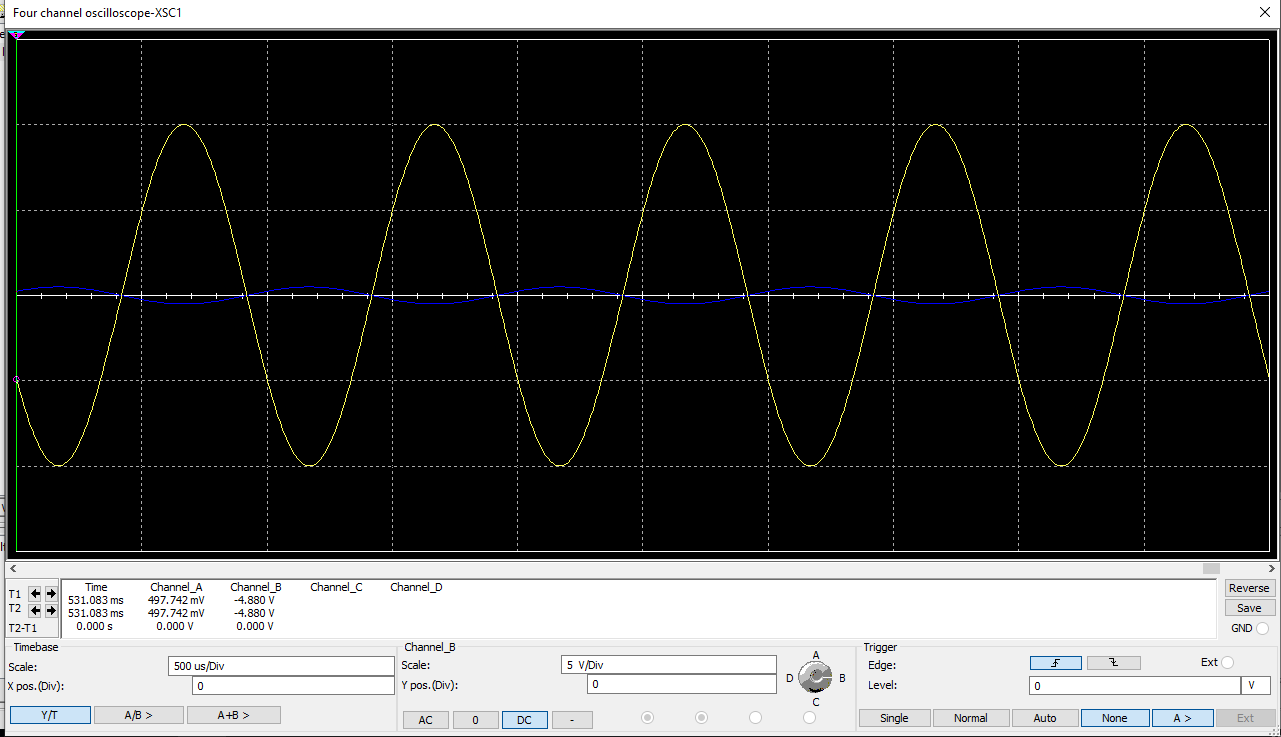
\includegraphics[scale=0.2]{aoinv.png}
    \caption{Amplificatore non invertente}
\end{figure}
\subsection{Tabella}
Valore misurato resistenze:\\
\begin{center}
        \begin{tabular}{|p{2cm}|p{2cm}|}
            \hline
            \rowcolor{RoyalBlue} $R_1$ & $R_2$ \\
            \hline
            \rowcolor{CornflowerBlue} $9.87k\Omega$ & $100k\Omega$  \\ 
            \hline
        \end{tabular}
        \label{Valore resistenze}
\end{center}
\noindent
Configurazione non invertente:\\
\begin{center}
    \begin{tabular}{|p{2cm} |p{2cm}|}
        \hline
        \rowcolor{RoyalBlue} $V_i$ & $V_o$  \\
        \hline
        \rowcolor{CornflowerBlue} $1.05V$ & $11V$  \\ 
        \hline
    \end{tabular}
    \label{Valore resistenze}
\end{center}

\noindent
Configurazione invertente:\\
\begin{center}
    \begin{tabular}{|p{2cm} |p{2cm}|}
        \hline
        \rowcolor{RoyalBlue} $V_i$ & $V_o$  \\
        \hline
        \rowcolor{CornflowerBlue} $1.06V$ & $12V$  \\ 
        \hline
    \end{tabular}
    \label{Valore resistenze}
\end{center}
\subsection{Commento dei dati raccolti in tabella}
I dati in tabella sono stati ottenuti misurando le grandezze riportate, rientrano nelle
tolleranze stabilite e sono rimasti stabili durante le misure.\\
\newpage
\section{Elaborazione dei dati raccolti}
\subsection{Calcoli}
Configurazione non invertente:\\
$A_v=1+\frac{R_1}{R_2}=1+\frac{100k\Omega}{10k\Omega}=11.2$\\
$A_{vmis}=\frac{V_o}{V_i}=\frac{11}{1.06}=1.65$\\
\\
\\
Configurazione invertente:\\
$A_v=-\frac{R_1}{R_2}=-\frac{100k\Omega}{10k\Omega}=-10.2$\\
$A_{vmis}=\frac{V_o}{V_i}=\frac{12}{1.05}=-10.43.$\\

\section{Analisi critica dei risultati e conclusioni}
Lo scopo è soddisfatto perché come si può evincere dai calcoli i valori del guadagno di tensione 
ottenuti in modo teorico e sperimentale corrispondono tollerate alcune discrepanze dati da errori
sistematici.\\
\end{document}